\documentclass[a4paper]{article}
\usepackage{polski}
\usepackage[T1]{fontenc}
\usepackage[polish]{babel}
\usepackage[utf8x]{inputenc}
\usepackage{amsmath}
\usepackage{graphicx}
\usepackage[T1]{fontenc}
\usepackage{lmodern}
\usepackage[top=1in, bottom=1.25in, left=1.25in, right=1.25in]{geometry}


\selectlanguage{polish}

\title{Portal społecznościowy}

\author{ Natalia Musiał \and Michał Juszczak \and Mariusz Nyznar\and  Agnieszka Kowal \and Łukasz Kmiecik \and Krzysztof Misiak}


\begin{document}
\maketitle


\section{Grupy}

Projekt zostanie zrealizowany przez 6 osób rozmieszczonych w trzech dwuosobowych grupach . 
\subsection{Zespół 1}
\begin{enumerate}
\item Natalia Musiał
\item Agnieszka Kowal
\end{enumerate}
\subsection{Zespół 2}
\begin{enumerate}
\item Łukasz Kmiecik
\item Michał Juszczak
\end{enumerate}
\subsection{Zespół 3}
\begin{enumerate}
\item Mariusz Nyznar
\item Krzysztof Misiak

\end{enumerate}


\section{Koncepcja systemu}

System ma być imitacją popularnego serwisu Twitter umożliwiającego komunikację pomiędzy użytkowanikami za pomocą krótkich wiadomości.
Możliwości systemu:
\begin{itemize}
\item Wysyłanie wiadomości między użytkownikami
\item Oznaczanie \#tagiem wpisów w celu szybszego ich wyszukiwania oraz poszerzania zasięgu wpływu
\item Oznaczanie @tagiem wpisów w celu oznaczenia innych użytkowników
\item Komentowanie postów przez innych użytkowników
\item Możliwość umieszczania adresów URL z filmikami
\item Możliwość umieszczania zdjęć 

\end{itemize}



\section{Technologie}
\begin{enumerate}
\item JPA (Hibernate) - ''Java Persistence Api'' to oficjalny standard mapowania obiektowo-relacyjnego (ORM) firmy Sun Microsystems dla języka programowania Java. Hibernate to framework do realizacji warstwy dostępu do danych (ang. persistence layer). Hibernate implementuje JPA.
\item REST - ''Representational State Transfer'' (zmiana stanu poprzez reprezentacje) to styl architektury oprogramowania wywiedziony z doświadczeń przy pisaniu specyfikacji protokołu HTTP dla systemów rozproszonych. 
\item JSF + Ajax - ''Java Server Faces'' to framework, bazujący na języku Java, który upraszcza tworzenie interfejsu użytkownika do aplikacji Java EE. ''Asynchronous JavaScript and XML'' to technika tworzenia aplikacji internetowych, w której interakcja użytkownika z serwerem odbywa się bez przeładowywania całego dokumentu, w sposób asynchroniczny.
\item EJB - ''Enterprise JavaBeans'' to komponenty pracujące po stronie serwera aplikacji, zawierające logikę biznesową.
\item CDI - ''Context and Dependency Injection''
\item Bean Validation 
\end{enumerate}



\section{Przypadki użycia}
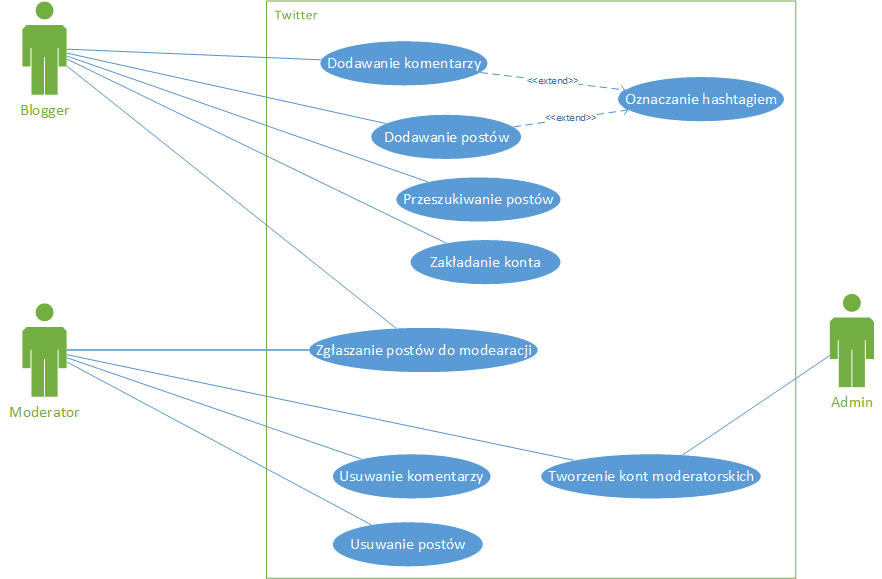
\includegraphics[width=\textwidth]{usecase}
\begin{tabular}{c p{10cm}}
Nazwa& Rejestracja	\\
Numer	& 1\\
Aktorzy & Użytkownik \\
Krótki opis & Użytkownik rejestruje nowe konto \\
Warunki wstępne&  aktywny adres e-mail\\
Warunki końcowe& Użytkownik uzyskuje dostęp do utworzonego konta\\
Główny przepływ zdarzeń&
\begin{enumerate} 
\item Użytkownik wybiera opcję ''\textbf{Zarejestruj}'' na stronie 
\item Przeglądarka wyświetla okno rejestracji nowego konta 
\item Użytkownik wpisuje nick, hasło oraz e-mail 
\item Przegląrka wyświetla komunikat o sukcesie oraz o wysłanym mailu aktywującym na podany adres email
\end{enumerate} \\
Alternatywny przebieg wydarzeń & 
3.a Przeglądrka wyświetla Podany nick istnieje w systemie \newline
3.a.1 Przeglądarka wyświetla komunikat z prośbą o wybranie innego nicka\newline
3.b Hasło ma niepoprawny format \newline
3.b.1 Przeglądarka wyświetla komunikat z prośbą o wpisanie hasła w żądanym formacie\newline
3.c Podany e-mail jest już w systemie \newline
3.c.1 Przeglądarka wyświetla komunikat o istnieniu adresu e-mail w systemie \newline
\\
\hline
\end{tabular}
\newline
\newline\\
\\

\begin{tabular}{c p{10cm}}
Nazwa&	Logowanie\\
Numer	& 2\\
Aktorzy &	Użytkownik\\
Krótki opis &  Użytkownik wpisuje swój nick oraz hasło w celu zalogowania\\
Warunki wstępne&	\\
Warunki końcowe&	Użytkownik uzyskuje dostęp do swojego konta\\
Główny przepływ zdarzeń&
\begin{enumerate}
\item Użytkownik wybiera opcję ''\textbf{Zaloguj}'' na stronie 
\item Przeglądarka wyświetla okno logowania
\item Użytkownik wpisuje swój nick oraz hasło
\item Przeglądarka wyświetla okno z potwierdzeniem logowania
\item Użytkownik uzyskuje dostęp do konta

\end{enumerate} \\
Alternatywny przebieg wydarzeń & 
4.a Użytkownik wpisuje niepoprawne hasło \newline
4.a.1 Przeglądarka wyświetla okno z komunikatem o niepoprawnym haśle \newline
4.a.2 Użytkownik wpisuje ponownie hasło\newline
\\
\hline
\end{tabular}
\newline
\newline


\begin{tabular}{c p{10cm}}
Nazwa&	Wpis\\
Numer	& 3\\
Aktorzy &	Użytkownik\\
Krótki opis &  Użytkownik dodaje wpis na tablicę\\
Warunki wstępne& Użytkownik jest zalogowany\\
Warunki końcowe& Wpis zostaje dodany na tablicę użytkownika, użytkownicy obserwujący mogą go zobaczyć na swoich tablicach\\
Główny przepływ zdarzeń&
\begin{enumerate}
\item Użytkownik wybiera opcję ''\textbf{Napisz nowego posta}'' 
\item Przeglądarka wyświetla okno nowego wpisu 
\item Użytkownik wpisuje tekst w oknie i wybiera opcję wysłania wpisu
\item Przeglądarka zamyka okno wpisu i przeładowuje stronę
\end{enumerate} \\

Alternatywny przebieg wydarzeń &
3.a Użytkownik wpisał zbyt wiele znaków \newline
3.a.1 Przeglądarka blokuje opcję wysłania wpisu i wyświetla komunikat o nadmiarze znaków \newline
3.a.2 Użytkownik skraca wpis \newline
3.a.3 Przeglądarka odblokowuje opcję wysłania \newline \\
\hline
\end{tabular}
\newline
\newline


\begin{tabular}{c p{10cm}}
Nazwa&	Szukanie wpisu po hashtagu\\
Numer	& 4\\
Aktorzy &	Użytkownik\\
Krótki opis &  Użytkownik klika na słowo oznaczone hashtagiem\\
Warunki wstępne& \\
Warunki końcowe& Przeglądarka wyświetla wszystkie wpisy zawierające dany hashtag, dodane przez znajomych użytkownika\\
Główny przepływ zdarzeń&
\begin{enumerate}
\item Użytkownik klina na słowo ze znakiem ''\textbf{\#}'' we wpisie na tablicy
\item Przeglądarka otwiera okno-nakładkę na tablicy oraz wyświetla wpisy zawierające dany hashtag
\end{enumerate} \\

Alternatywny przebieg wydarzeń &
2.a Brak wpisów z danym hashtagiem \newline
2.a.1 Przeglądarka wyświetla okno-nakładkę na tablicy oraz wyświetla komunikat ''\textbf{Brak wpisów dla <hashtag>}'' \newline \\
\hline
\end{tabular}
\newline
\newline
\begin{tabular}{c p{10cm}}
Nazwa&	Wyświetlenie profilu\\
Numer	& 5\\
Aktorzy &	Użytkownik\\
Krótki opis &  Użytkownik wybiera profil do obejrzenia\\
Warunki wstępne& \\
Warunki końcowe& Zostaje wyświetlony profil wybranego użytkownika wraz z tablicą wpisów\\
Główny przepływ zdarzeń&
\begin{enumerate}
\item Użytkownik klika na profil, który chce obejrzeć 
\item Przeglądarka wyświetla główny profil danego użytkownika wraz z tablicą wpisów
\end{enumerate} \\

Alternatywny przebieg wydarzeń & \\
\hline
\end{tabular}
\newline
\newline
\begin{tabular}{c p{10cm}}
Nazwa&	Edycja konta\\
Numer	& 6\\
Aktorzy &	Użytkownik\\
Krótki opis &  Zmiana informacji profilu użytkownika\\
Warunki wstępne& \\
Warunki końcowe& Dane są zatwierdzone i zmienione\\
Główny przepływ zdarzeń&
\begin{enumerate}
\item Użytkownik wybiera opcję ''\textbf{Edytuj profil}'' pod zdjęciem profilowym
\item Przeglądarka otwiera okno profilu z odblokowaną możliwością edycji
\item Użytkownik wpisuje nowe dane do wybranego pola tekstowego
\item Przeglądarka wyświetla znak poprawności formatu obok danego pola
\item Użytkownik wybiera opcję ''\textbf{Zatwierdź zmiany}'' 
\item Przeglądarka otwiera okno strony głównej
\end{enumerate} \\

Alternatywny przebieg wydarzeń & 
4.a Niepoprawny format pola tekstowego \newline
4.a.1 Przeglądarka wyświetla znak niepoprawnego formatu obok danego pola \newline
4.a.2 Użytkownik poprawia dane w polu tekstowym\newline
4.a.3 Przejście do kroku 4\newline 
5.a Użytkownik wybiera opcję ''\textbf{Anuluj}'' \newline
5.a. Przejście do kroku 6 \newline \\
\hline
\end{tabular}
\newline
\newline
\begin{tabular}{c p{10cm}}
Nazwa&	Szukanie użytkownika po tagu\\
Numer	& 7\\
Aktorzy &	Użytkownik\\
Krótki opis &  Uzytkownik klika na nick oznaczony tagiem\\
Warunki wstępne& \\
Warunki końcowe& Zostaje otwarty profil wybranego użytkownika\\
Główny przepływ zdarzeń&
\begin{enumerate}
\item Użytkownik klika na tekst \@''<nick>''
\item Przeglądarka otwiera okno z profilem wybranego użytkownika wraz z tablicą wpisów
\end{enumerate} \\

Alternatywny przebieg wydarzeń &  \\
\hline
\end{tabular}
\newline
\newline
\begin{tabular}{c p{10cm}}
Nazwa& Odświeżenie strony\\
Numer	& 8\\
Aktorzy &	Użytkownik\\
Krótki opis & Załądowanie nowych wiadomości na tablicy\\
Warunki wstępne& \\
Warunki końcowe& Na tablicy wpisów pojawiają się nowe wpisy\\
Główny przepływ zdarzeń&
\begin{enumerate}
\item Użytkownik wybiera ikonę odświeżenia tablicy
\item Przeglądarka doładowuje nowe wpisy na tablicy od góry
\end{enumerate} \\

Alternatywny przebieg wydarzeń & 
2.a Brak nowych wpisów \newline 
2.a.1 Przeglądarka wyświetla dotychczasowy stan tablicy
\\
\hline
\end{tabular}
\newline
\newline
\begin{tabular}{c p{10cm}}
Nazwa& Usunięcie wpisu\\
Numer	& 9\\
Aktorzy &	Użytkownik\\
Krótki opis & Usunięcie dodanego wpisu z tablicy\\
Warunki wstępne& Użytkownik jest autorem wpisu\\
Warunki końcowe& Wpis znika z tablicy wpisów\\
Główny przepływ zdarzeń&
\begin{enumerate}
\item Użytkownik wybiera opcję ''\textbf{Usuń wpis}'' w okienku wpisu
\item Przeglądarka wyświetla okno dialogowe z prośbą o potwierdzenie
\item Użytkownik wybiera opcję ''\textbf{Usuń}''
\item Przeglądarka wyświetla stronę główną bez wybranego wpisu
\end{enumerate} \\

Alternatywny przebieg wydarzeń & 
3.a Użytkownik wybiera opcję ''\textbf{Anuluj}'' \newline 
3.a.1 Przeglądarka wyświetla stronę główną z wpisem
\\
\hline
\end{tabular}

\begin{tabular}{c p{10cm}}
Nazwa& Edytuj wpisu\\
Numer	& 9\\
Aktorzy &	Użytkownik\\
Krótki opis & Usunięcie dodanego wpisu z tablicy\\
Warunki wstępne& Użytkownik jest autorem wpisu\\
Warunki końcowe& Wpis znika z tablicy wpisów\\
Główny przepływ zdarzeń&
\begin{enumerate}
\item Użytkownik wybiera opcję ''\textbf{Usuń wpis}'' w okienku wpisu
\item Przeglądarka wyświetla okno dialogowe z prośbą o potwierdzenie
\item Użytkownik wybiera opcję ''\textbf{Usuń}''
\item Przeglądarka wyświetla stronę głównąbez wybranego wpisu
\end{enumerate} \\

Alternatywny przebieg wydarzeń & 
3.a Użytkownik wybiera opcję ''\textbf{Anuluj}'' \newline 
3.a.1 Przeglądarka wyświetla stronę główną z wpisem
\\
\hline
\end{tabular}


\section{Zarys architektury systemu}
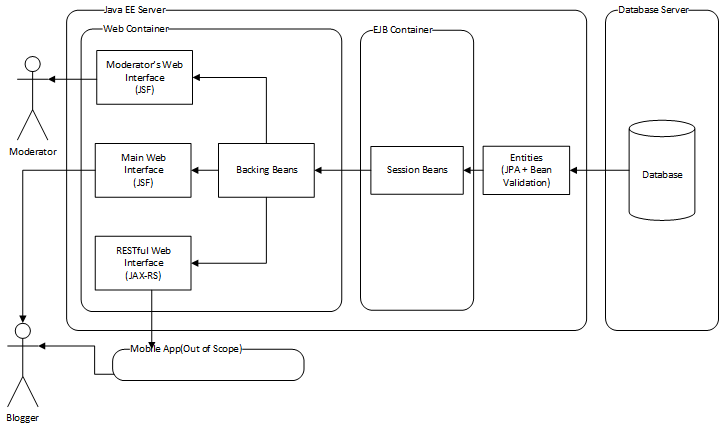
\includegraphics[width=\textwidth]{architecture}

\section{Schemat bazy danych}
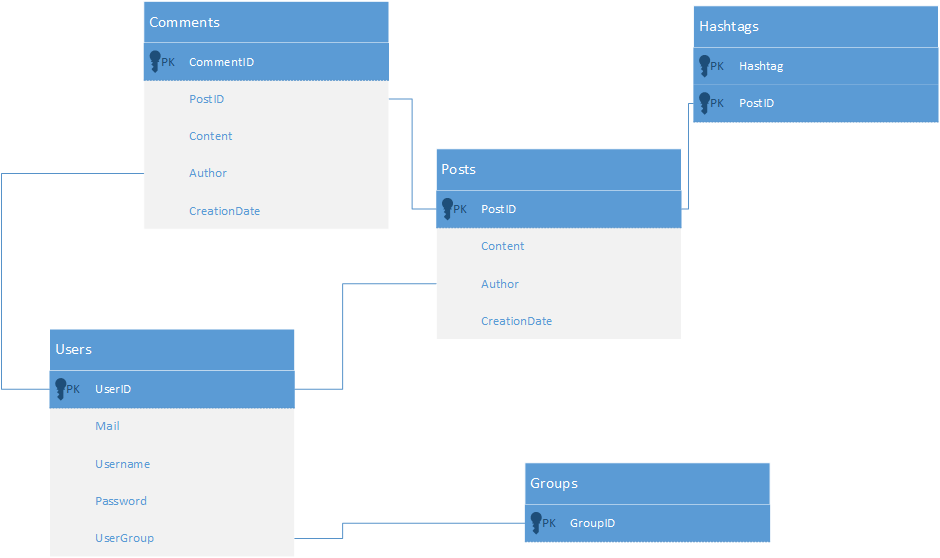
\includegraphics[width=\textwidth]{database}

\section{Lista serwisów}
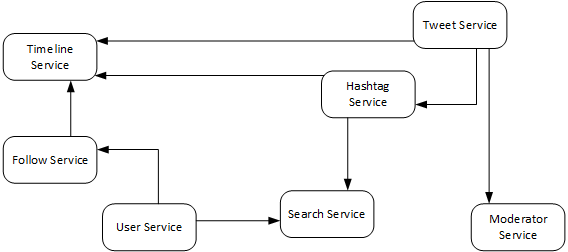
\includegraphics[width=\textwidth]{services}
\begin{itemize}
\item{Timeline Service - przygotowuje listę tweetów do wyświetlenia konkretnemu użytkownikowi na podstawie danych o nim}
\item{Search Service - odpowiada za wyszukiwanie tweetów, tagów, użytkowników}
\item{Tweet Service - tworzenie nowych tweetów, dostarczanie tweetów}
\item{User Service - dodawanie, edycja kont użytkowników}
\item{Direct Message Service - przesyłanie wiadomości bezpośrednich między użytkownikami}
\item{Moderator Service - udostępnia moderatorom możliwość przeglądania kolejki zgłoszeń, odpowiadania na zgłoszenia}
\item{Follow Service - odpowiada za "śledzenie" działań jednych bloggerów przez innych}
\item{Hashtag Service - odpowiada za utrzymywanie powiązań pomiędzy postami a tagami}

\end{itemize}

\section{Podział pracy}

Presentation Layer:

\begin{itemize}
\item {REST API - Team 1, 2, 3}
\item {WEB API - Team 1, 2, 3}
\item {Frontend - Team 1}
\end{itemize}

Services:

\begin{itemize}
\item {Tweet Service - Team 3}
\item {User Service - Team 2 }
\item {Search Service - Team 1}
\item {Timeline Service - Team 3}
\item {Hashtag Service - Team 2}
\item {Follow Service - Team 1}
\item {Moderator Service - Team 3}
\end{itemize}
\end{document}

















